% This is the Reed College LaTeX thesis template. Most of the work
% for the document class was done by Sam Noble (SN), as well as this
% template. Later comments etc. by Ben Salzberg (BTS). Additional
% restructuring and APA support by Jess Youngberg (JY).
% Your comments and suggestions are more than welcome; please email
% them to cus@reed.edu
%
% See https://www.reed.edu/cis/help/LaTeX/index.html for help. There are a
% great bunch of help pages there, with notes on
% getting started, bibtex, etc. Go there and read it if you're not
% already familiar with LaTeX.
%
% Any line that starts with a percent symbol is a comment.
% They won't show up in the document, and are useful for notes
% to yourself and explaining commands.
% Commenting also removes a line from the document;
% very handy for troubleshooting problems. -BTS

% As far as I know, this follows the requirements laid out in
% the 2002-2003 Senior Handbook. Ask a librarian to check the
% document before binding. -SN

%%
%% Preamble
%%
% \documentclass{<something>} must begin each LaTeX document
\documentclass[12pt,twoside]{reedthesis}
% Packages are extensions to the basic LaTeX functions. Whatever you
% want to typeset, there is probably a package out there for it.
% Chemistry (chemtex), screenplays, you name it.
% Check out CTAN to see: https://www.ctan.org/
%%
\usepackage{graphicx,latexsym}
\usepackage{amsmath}
\usepackage{amssymb,amsthm}
\usepackage{longtable,booktabs,setspace}
\usepackage{chemarr} %% Useful for one reaction arrow, useless if you're not a chem major
\usepackage[hyphens]{url}
% Added by CII
\usepackage{hyperref}
\usepackage{lmodern}
\usepackage{float}
\floatplacement{figure}{H}
% Thanks, @Xyv
\usepackage{calc}
% End of CII addition
\usepackage{rotating}

% Next line commented out by CII
%%% \usepackage{natbib}
% Comment out the natbib line above and uncomment the following two lines to use the new
% biblatex-chicago style, for Chicago A. Also make some changes at the end where the
% bibliography is included.
%\usepackage{biblatex-chicago}
%\bibliography{thesis}


% Added by CII (Thanks, Hadley!)
% Use ref for internal links
\renewcommand{\hyperref}[2][???]{\autoref{#1}}
\def\chapterautorefname{Chapter}
\def\sectionautorefname{Section}
\def\subsectionautorefname{Subsection}
% End of CII addition

% Added by CII
\usepackage{caption}
\captionsetup{width=5in}
% End of CII addition

% \usepackage{times} % other fonts are available like times, bookman, charter, palatino

% Syntax highlighting #22

% To pass between YAML and LaTeX the dollar signs are added by CII
\title{Short-Term Price Elasticities of Heating Demand: A Statistical Analysis of Consumption Data in Germany}
\author{Marc Blauert}
% The month and year that you submit your FINAL draft TO THE LIBRARY (May or December)
\date{2021-12-12}
\division{Albrecht Daniel Thaer-Institute}
\advisor{Prof.~Dr.~Karsten Neuhoff}
\institution{Humboldt University of Berlin}
\degree{Master of Science}
%If you have two advisors for some reason, you can use the following
% Uncommented out by CII
\altadvisor{Prof.~Dr.~Tobias Krüger}
% End of CII addition

%%% Remember to use the correct department!
\department{Integrated Natural Resource Management (INRM)}
% if you're writing a thesis in an interdisciplinary major,
% uncomment the line below and change the text as appropriate.
% check the Senior Handbook if unsure.
%\thedivisionof{The Established Interdisciplinary Committee for}
% if you want the approval page to say "Approved for the Committee",
% uncomment the next line
%\approvedforthe{Committee}

% Added by CII
%%% Copied from knitr
%% maxwidth is the original width if it's less than linewidth
%% otherwise use linewidth (to make sure the graphics do not exceed the margin)
\makeatletter
\def\maxwidth{ %
  \ifdim\Gin@nat@width>\linewidth
    \linewidth
  \else
    \Gin@nat@width
  \fi
}
\makeatother

% From {rticles}
\newlength{\csllabelwidth}
\setlength{\csllabelwidth}{3em}
\newlength{\cslhangindent}
\setlength{\cslhangindent}{1.5em}
% for Pandoc 2.8 to 2.10.1
\newenvironment{cslreferences}%
  {}%
  {\par}
% For Pandoc 2.11+
% As noted by @mirh [2] is needed instead of [3] for 2.12
\newenvironment{CSLReferences}[2] % #1 hanging-ident, #2 entry spacing
 {% don't indent paragraphs
  \setlength{\parindent}{0pt}
  % turn on hanging indent if param 1 is 1
  \ifodd #1 \everypar{\setlength{\hangindent}{\cslhangindent}}\ignorespaces\fi
  % set entry spacing
  \ifnum #2 > 0
  \setlength{\parskip}{#2\baselineskip}
  \fi
 }%
 {}
\usepackage{calc} % for calculating minipage widths
\newcommand{\CSLBlock}[1]{#1\hfill\break}
\newcommand{\CSLLeftMargin}[1]{\parbox[t]{\csllabelwidth}{#1}}
\newcommand{\CSLRightInline}[1]{\parbox[t]{\linewidth - \csllabelwidth}{#1}}
\newcommand{\CSLIndent}[1]{\hspace{\cslhangindent}#1}

\renewcommand{\contentsname}{Table of Contents}
% End of CII addition

\setlength{\parskip}{0pt}

% Added by CII

\providecommand{\tightlist}{%
  \setlength{\itemsep}{0pt}\setlength{\parskip}{0pt}}

\Acknowledgements{
People I need to thank: Franziska, Till, Abteilung beim DIW --\textgreater{} Bereitstellung Daten, Betreuer.
}

\Dedication{

}

\Preface{

}

\Abstract{
The preface pretty much says it all.

\par

Second paragraph of abstract starts here.
}

	\usepackage{setspace}\onehalfspacing
	\usepackage{booktabs}
 \usepackage{longtable}
 \usepackage{array}
 \usepackage{multirow}
 \usepackage{wrapfig}
 \usepackage{float}
 \usepackage{colortbl}
 \usepackage{pdflscape}
 \usepackage{tabu}
 \usepackage{threeparttable}
 \usepackage{threeparttablex}
 \usepackage[normalem]{ulem}
 \usepackage{makecell}
 \usepackage{xcolor}
% End of CII addition
%%
%% End Preamble
%%
%
\begin{document}

% Everything below added by CII
  \maketitle

\frontmatter % this stuff will be roman-numbered
\pagestyle{empty} % this removes page numbers from the frontmatter
  \begin{acknowledgements}
    People I need to thank: Franziska, Till, Abteilung beim DIW --\textgreater{} Bereitstellung Daten, Betreuer.
  \end{acknowledgements}

  \hypersetup{linkcolor=black}
  \setcounter{secnumdepth}{2}
  \setcounter{tocdepth}{2}
  \tableofcontents

  \listoftables

  \listoffigures
  \begin{abstract}
    The preface pretty much says it all.

    \par

    Second paragraph of abstract starts here.
  \end{abstract}

\mainmatter % here the regular arabic numbering starts
\pagestyle{fancyplain} % turns page numbering back on

\hypertarget{introduction}{%
\chapter{Introduction}\label{introduction}}
\begin{figure}

{\centering 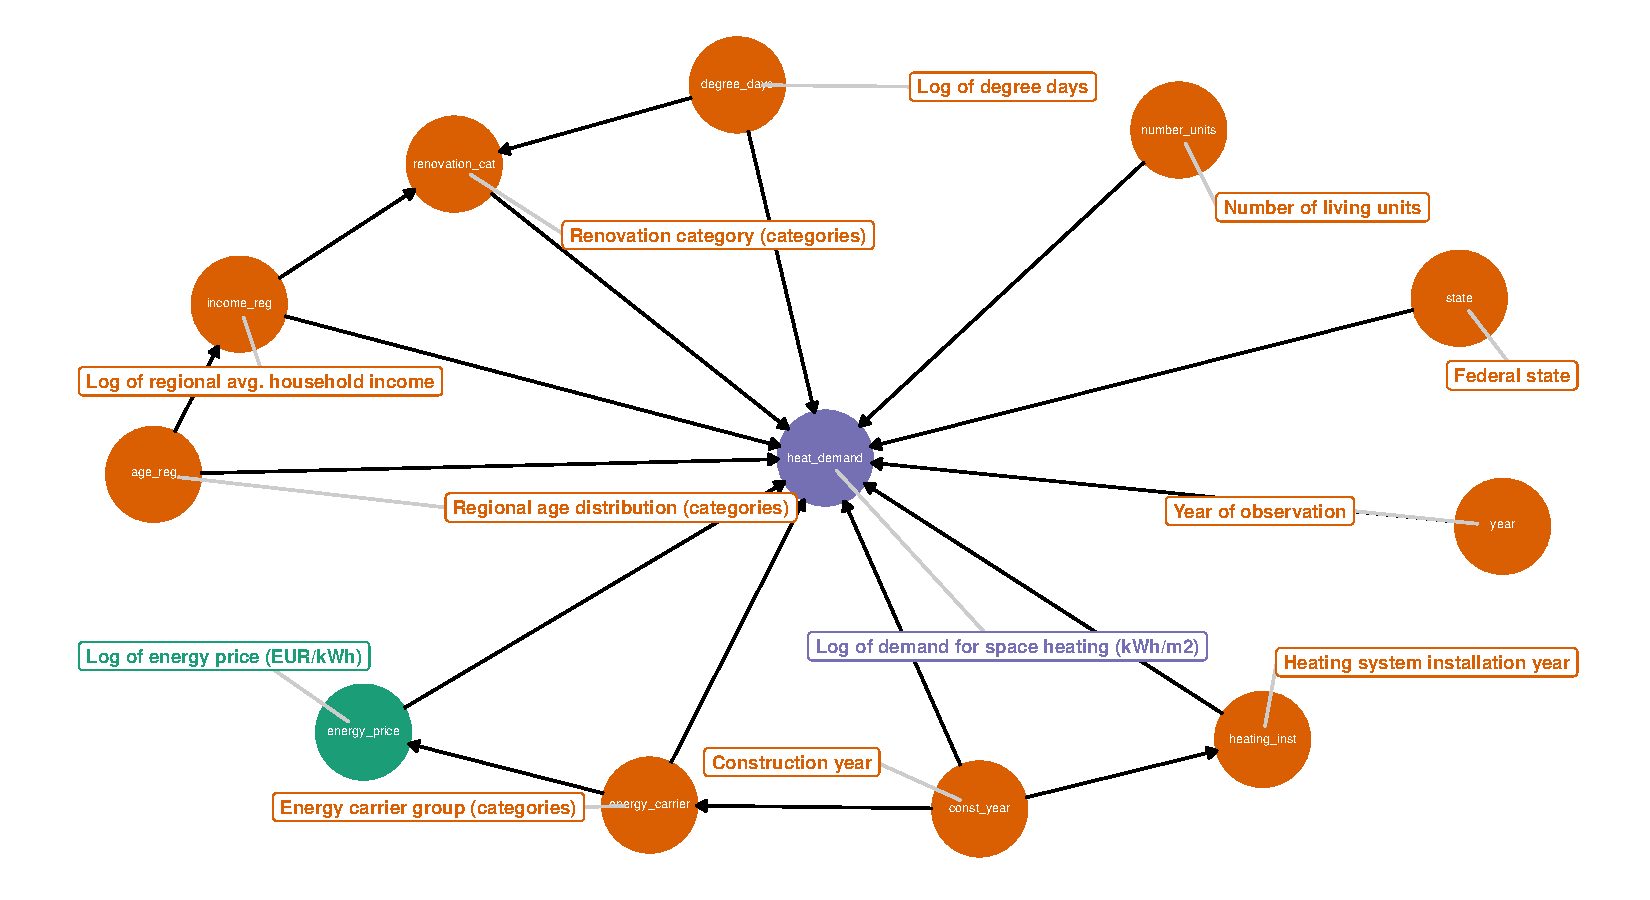
\includegraphics[width=1\linewidth]{figure/conceptual_dag} 

}

\caption{DAG}\label{fig:dag}
\end{figure}
This is to test citations \protect\hyperlink{ref-asche_etal08}{Asche, Bjarte Nilsen, \& Tveteras} (\protect\hyperlink{ref-asche_etal08}{2008}).

\hypertarget{literature}{%
\chapter{Literature Review}\label{literature}}

\hypertarget{methods}{%
\chapter{Methods}\label{methods}}

\hypertarget{data}{%
\chapter{Data}\label{data}}

\hypertarget{results}{%
\chapter{Results}\label{results}}

\begingroup\fontsize{10}{12}\selectfont
\begin{longtable}[t]{lr}
\caption{\label{tab:tabletest}Number of flight connections per destination}\\
\toprule
Destination & Number of connections\\
\midrule
\endfirsthead
\caption[]{\label{tab:tabletest}Number of flight connections per destination \textit{(continued)}}\\
\toprule
Destination & Number of connections\\
\midrule
\endhead

\endfoot
\bottomrule
\multicolumn{2}{l}{\rule{0pt}{1em}\textsuperscript{1} This table was created based on the flights dataset.}\\
\multicolumn{2}{l}{\rule{0pt}{1em}\textsuperscript{2} Source: R Packages.}\\
\endlastfoot
Albuquerque International Sunport & 30\\
Bob Hope & 261\\
Boise Air Terminal & 29\\
Charlotte Douglas Intl & 45\\
Chicago Midway Intl & 104\\
\addlinespace
Chicago Ohare Intl & 524\\
Dallas Fort Worth Intl & 441\\
Denver Intl & 905\\
Detroit Metro Wayne Co & 55\\
General Edward Lawrence Logan Intl & 70\\
\addlinespace
George Bush Intercontinental & 228\\
Hartsfield Jackson Atlanta Intl & 410\\
Honolulu Intl & 180\\
John F Kennedy Intl & 137\\
John Wayne Arpt Orange Co & 247\\
\addlinespace
Kahului & 171\\
Kansas City Intl & 89\\
Klamath Falls Airport & 82\\
Kona Intl At Keahole & 90\\
Lihue & 52\\
\addlinespace
Long Beach & 263\\
Los Angeles Intl & 912\\
Mahlon Sweet Fld & 189\\
Mc Carran Intl & 564\\
Metropolitan Oakland Intl & 451\\
\addlinespace
Minneapolis St Paul Intl & 270\\
Newark Liberty Intl & 91\\
Norman Y Mineta San Jose Intl & 574\\
Ontario Intl & 196\\
Palm Springs Intl & 105\\
\addlinespace
Phoenix Sky Harbor Intl & 888\\
Reno Tahoe Intl & 94\\
Roberts Fld & 252\\
Ronald Reagan Washington Natl & 87\\
Sacramento Intl & 404\\
\addlinespace
Salt Lake City Intl & 538\\
San Diego Intl & 265\\
San Francisco Intl & 1265\\
Santa Barbara Muni & 89\\
Seattle Tacoma Intl & 569\\
\addlinespace
Ted Stevens Anchorage Intl & 254\\
Tucson Intl & 90\\
Washington Dulles Intl & 89\\*
\end{longtable}
\endgroup{}

\hypertarget{discussion}{%
\chapter{Discussion}\label{discussion}}

\hypertarget{conclusion}{%
\chapter{Conclusion}\label{conclusion}}

\appendix

\hypertarget{first-appendix}{%
\chapter{First Appendix}\label{first-appendix}}

\hypertarget{second-appendix}{%
\chapter{Second Appendix}\label{second-appendix}}

(\ldots)

\backmatter

\hypertarget{references}{%
\chapter*{References}\label{references}}
\addcontentsline{toc}{chapter}{References}

\markboth{References}{References}

\noindent

\setlength{\parindent}{-0.20in}

\hypertarget{refs}{}
\begin{CSLReferences}{1}{0}
\leavevmode\vadjust pre{\hypertarget{ref-asche_etal08}{}}%
Asche, F., Bjarte Nilsen, O., \& Tveteras, R. (2008). Natural Gas Demand in the European Household Sector. \emph{The Energy Journal}, \emph{29}(3). http://doi.org/\href{https://doi.org/10.5547/ISSN0195-6574-EJ-Vol29-No3-2}{10.5547/ISSN0195-6574-EJ-Vol29-No3-2}

\end{CSLReferences}

% Index?

\end{document}
